\documentclass[12pt,a4paper]{article}

\usepackage[utf8]{inputenc}
\usepackage[T1]{fontenc}
\usepackage[english]{babel}
\usepackage{amsmath, amsthm, amssymb}
\usepackage{geometry}
\usepackage{booktabs}
\usepackage{array}
\usepackage{longtable}
\usepackage{pgfplots}
\pgfplotsset{compat=1.18}
\usepackage{xcolor}
\usepackage{hyperref}
\usepackage{listings}
\usepackage{caption}
\usepackage{subcaption}
\usepackage{graphicx}
\usepackage{float}
% Use standard paragraph formatting: justified text with indentation.
\setlength{\parindent}{1em}
\setlength{\parskip}{0pt}
\usepackage{titlesec}
\usepackage{enumitem}
\usepackage[square,numbers]{natbib}

\geometry{
  top=2.5cm, bottom=2.5cm,
  left=2.5cm, right=2.5cm
}

\hypersetup{
  colorlinks=true,
  linkcolor=blue!60!black,
  citecolor=blue!60!black,
  urlcolor=blue!60!black
}

\lstset{
  language=C,
  basicstyle=\ttfamily\small,
  keywordstyle=\bfseries\color{blue!70!black},
  commentstyle=\itshape\color{green!50!black},
  stringstyle=\color{red!60!black},
  numbers=left,
  numberstyle=\tiny\color{gray},
  numbersep=6pt,
  frame=single,
  breaklines=true,
  tabsize=4
}

\theoremstyle{definition}
\newtheorem{definition}{Definition}[section]
\newtheorem{theorem}{Theorem}[section]
\newtheorem{proposition}{Proposition}[section]

% ─── Title and Author ─────────────────────────────────────────────────────────
\title{\textbf{A Comparative Empirical Analysis of Sorting Algorithms\\
Under Varied Input Distributions}}

\author{
  Daniel Pantea \\
  \small Faculty of Informatics, Department of Computer Science \\
  \small West University of Timișoara \\
  \small \href{mailto:daniel.pantea06@e-uvt.ro}{daniel.pantea06@e-uvt.ro}
  \small \href{https://github.com/Pantea-Daniel}{https://github.com/Pantea-Daniel}
}

\date{\today}

\begin{document}

\maketitle
\thispagestyle{empty}

% ─── Abstract ─────────────────────────────────────────────────────────────────
\begin{abstract}
Almost every software system depends on sorting at some point --- whether it is ranking search results, scheduling tasks, or looking up records in a database. Even though sorting has been studied for a long time, choosing the right algorithm for a specific situation is still not simple. The reason is that theoretical complexity alone does not tell the full story. How fast an algorithm runs also depends on the shape of the input data. This paper studies that question for six well-known sorting algorithms: Bubble Sort, Insertion Sort, Selection Sort, Quick Sort, Merge Sort, and Radix Sort.

Instead of testing only fully random or fully reversed arrays, we also test \emph{partially sorted} arrays. These are arrays that start in order but then have a controlled number of random swaps applied. We test seven different input sizes, from 10 to 1\,000\,000 elements, and repeat each test many times to get stable timing results. We measure how long each sort takes in milliseconds.

The results show some surprising findings. Insertion Sort, which is usually seen as a slow $O(n^2)$ algorithm, can be as fast as Quick Sort when the data is nearly sorted. Radix Sort is the fastest at large sizes on random data, finishing one million elements in under 100 ms. Merge Sort is the most consistent --- its speed barely changes no matter what kind of input it receives. These findings give clear, practical advice on which algorithm to choose depending on the situation.
\end{abstract}

\newpage
\tableofcontents
\newpage

% ─── 1. Introduction ──────────────────────────────────────────────────────────
\section{Introduction}

\subsection{Organization of the Paper}

The background theory in this paper is based on well-known sources listed in Section~\ref{sec:related}. The original work done by the author includes: (1) designing and writing the C benchmarking program, including the function that creates partially sorted arrays with a chosen level of disorder; (2) running tests across seven input sizes, six algorithms, and seven input types; and (3) studying how the order of the input affects the speed of each algorithm, with a focus on Insertion Sort and Bubble Sort on partially sorted data.

Section~\ref{sec:formal} gives formal definitions and explains the complexity of each algorithm. Section~\ref{sec:implementation} describes how the program was built and how the data structures work. Section~\ref{sec:experiments} explains the test setup and shows the results. Section~\ref{sec:related} reviews related work done by others. Section~\ref{sec:conclusions} summarizes the main findings and suggests ideas for future work. Section~\ref{sec:bibliography} lists all sources used.

% ─── 2. Formal Presentation ───────────────────────────────────────────────────
\section{Problem Formulation and Algorithmic Approaches}
\label{sec:formal}

\subsection{Problem Definition}

\begin{definition}[Sorting Problem]\cite{knuth1998,cormen2022}
Given a sequence $A = (a_1, a_2, \ldots, a_n)$ of $n$ elements drawn from a totally ordered set $(S, \leq)$, produce a permutation $A' = (a_{\pi(1)}, a_{\pi(2)}, \ldots, a_{\pi(n)})$ such that $a_{\pi(i)} \leq a_{\pi(i+1)}$ for all $1 \leq i < n$.
\end{definition}

In this paper, $S = \mathbb{Z}$ and all comparisons are done on 32-bit signed integers.

\begin{definition}[Inversion Count]\cite{cormen2022,knuth1998}
For a sequence $A$ of length $n$, the inversion count is $\text{inv}(A) = |\{(i,j) : i < j \text{ and } a_i > a_j\}|$. A fully sorted array has $\text{inv}(A) = 0$; a fully reversed array has $\text{inv}(A) = \binom{n}{2}$.
\end{definition}

The inversion count is a way to measure how unsorted an array is. Algorithms that directly depend on this count (such as Insertion Sort) will run faster when the count is low.

\subsection{Algorithm Descriptions and Complexity}

\paragraph{Bubble Sort.}
Goes through the array repeatedly, swapping two neighbouring elements if they are in the wrong order. It stops early if a full pass made no swaps. Best case is $\Theta(n)$ (already sorted), worst case is $\Theta(n^2)$ (fully reversed). The total number of swaps equals $\text{inv}(A)$.

\paragraph{Insertion Sort.}
Keeps a sorted section at the start of the array, and places each new element into the correct position by shifting elements one step to the right. Its running time is $\Theta(n + \text{inv}(A))$ --- this means it is very fast on nearly sorted data and slow on reversed data. It also accesses memory in order, which is good for cache performance.

\paragraph{Selection Sort.}
Finds the smallest element in the unsorted part of the array and puts it at the front. The number of comparisons is always $\Theta(n^2)$, no matter what the input looks like. Only the number of swaps changes. This means its speed is not affected by the order of the input.

\paragraph{Quick Sort.}
Splits the array around a chosen pivot element and sorts each part separately using recursion. This implementation uses median-of-three pivot selection:

\begin{definition}[Median-of-Three Pivot]\cite{sedgewick2011}
Given indices $\ell$, $m = \lfloor(\ell + r)/2\rfloor$, and $r$, sort $\{A[\ell], A[m], A[r]\}$ in place and use $A[r]$ (the median) as the pivot.
\end{definition}

\begin{theorem}
Quick Sort with median-of-three achieves an expected $O(n \log n)$ number of comparisons on random input and avoids the $O(n^2)$ worst case that happens with a naive pivot on already-sorted or reversed arrays.
\end{theorem}

\paragraph{Merge Sort.}
Splits the array into two halves, sorts each half, and then joins them back together in order. Its time complexity is $\Theta(n \log n)$ in all cases. It needs $\Theta(n)$ extra memory for the merge step. Because the merge step does not depend on the order of the input, Merge Sort behaves the same way no matter what data it receives.

\paragraph{Radix Sort.}
Does not use comparisons. Instead, it sorts integers digit by digit, starting from the least significant digit, using a stable counting sort at each step. With $d$ digits in base $b$:

\begin{proposition}
Radix Sort runs in $\Theta(d(n + b))$ time and uses $\Theta(n + b)$ extra memory. For integers of fixed size in base 10, $d = \lfloor\log_{10}(\max A)\rfloor + 1$, which means it behaves like $O(n)$ for bounded integer values.
\end{proposition}

\subsection{Summary of Theoretical Complexity}

Table~\ref{tab:complexity} summarizes the time and space complexity of the six algorithms discussed in this section.

\begin{table}[H]
\centering
\caption{Theoretical time complexity of the six algorithms.}
\label{tab:complexity}
\begin{tabular}{lcccc}
\toprule
\textbf{Algorithm} & \textbf{Best Case} & \textbf{Average Case} & \textbf{Worst Case} & \textbf{Space} \\
\midrule
Bubble Sort      & $\Theta(n)$        & $\Theta(n^2)$         & $\Theta(n^2)$       & $O(1)$ \\
Insertion Sort   & $\Theta(n)$        & $\Theta(n^2)$         & $\Theta(n^2)$       & $O(1)$ \\
Selection Sort   & $\Theta(n^2)$      & $\Theta(n^2)$         & $\Theta(n^2)$       & $O(1)$ \\
Quick Sort       & $\Theta(n \log n)$ & $\Theta(n \log n)$    & $\Theta(n^2)$*      & $O(\log n)$ \\
Merge Sort       & $\Theta(n \log n)$ & $\Theta(n \log n)$    & $\Theta(n \log n)$  & $O(n)$ \\
Radix Sort       & $\Theta(dn)$       & $\Theta(dn)$          & $\Theta(dn)$        & $O(n+b)$ \\
\bottomrule
\multicolumn{5}{l}{\footnotesize *Mitigated by median-of-three pivot in this implementation.}
\end{tabular}
\end{table}

% ─── 3. Implementation ────────────────────────────────────────────────────────
\section{Implementation and Architecture}
\label{sec:implementation}

\subsection{Architecture Overview}

The benchmark is written as a single C file, compiled with GCC. The code is split into four clear parts:

\begin{enumerate}[label=\arabic*.]
  \item \textbf{Data generation}: Functions \texttt{generateIntArray}, \texttt{generateReverseSortedIntArray}, and \texttt{generatePartiallySortedIntArray} create the test arrays.
  \item \textbf{Sorting functions}: One function per algorithm, each working directly on the input array.
  \item \textbf{Timing loop}: \texttt{analyzeSortAlg} runs each algorithm many times, using \texttt{memcpy} to reset the array to its original state before each run.
  \item \textbf{Output}: Results are saved to both the terminal and a CSV file.
\end{enumerate}

\subsection{Data Structures}

All arrays are stored on the heap using \texttt{malloc} and freed with \texttt{free}. The timing loop keeps a \emph{master} copy of the original array (which is never changed) and a \emph{working} copy that is reset before each timed run. This makes sure every run starts with exactly the same data. Time is measured using the \texttt{clock()} function, which gives CPU time in milliseconds.

\subsection{Partial Sort Generator}

One of the new features of this benchmark is the partially sorted input generator. It builds an ordered array and then makes a controlled number of random swaps to introduce disorder. The number of swaps is $n / \text{factor}$, so a smaller factor creates more disorder and a larger factor keeps the array closer to sorted. Short pseudocode for this generator appears in Appendix~\ref{app:pseudocode}.

\subsection{Median-of-Three Quick Sort}

The pivot selection function works as follows. It looks at the first, middle, and last elements of the current subarray, sorts those three values using simple comparisons, and places the middle value at the end to use as the pivot. This helps avoid the worst case on already-sorted or reversed arrays. A short pseudocode sketch is available in Appendix~\ref{app:pseudocode}.

\subsection{User Manual}

This section gives a brief and simple guide to compile and run the benchmark.

\subsubsection*{Prerequisites}

The benchmark requires only a C99-compatible compiler and the standard C library. No extra libraries are needed. The tools used for the original tests were:

\begin{itemize}[noitemsep]
  \item \textbf{GCC} (version 7 or later), or another C99 compiler such as MSVC or Clang.
  \item \textbf{CMake} (version 3.10 or later), which was used to produce the release build in the original study.
  \item A terminal or command prompt where the program can write the output file \texttt{results1.csv}.
\end{itemize}

\subsubsection*{Building and Running}

Compile the program in release mode and then run the executable. On Windows, the output is typically \texttt{sorting\_algorithms.exe}. The benchmark runs automatically with no command-line arguments and writes the results to a CSV file.

\subsubsection*{Configuration}

All experimental settings are controlled from the \texttt{main()} function. You can change the input sizes, repetition counts, and output file name in one place. The default benchmark is set up so that small inputs run many times for accuracy and large inputs run once to keep total execution time reasonable.

\subsubsection*{Output Format}

The program writes results both to the terminal and to \texttt{results1.csv}. Each row contains the number of elements, the number of runs, the algorithm name, the input variant, the average elapsed time in milliseconds, and a short summary message.

\subsubsection*{Interpreting the Results}

The output is designed to be easy to read. For example, one line reports how long Quick Sort took on a random array of 1\,000 elements. The benchmark uses more repetitions for small sizes to ensure the measured time is meaningful.

% ─── 4. Experiments ───────────────────────────────────────────────────────────
\section{Experimental Evaluation}
\label{sec:experiments}

\subsection{Experimental Setup}

\begin{itemize}[noitemsep]
  \item \textbf{Platform}: Windows 10, compiled with GCC via CMake (Release mode).
  \item \textbf{Input sizes}: $n \in \{10,\, 50,\, 100,\, 1000,\, 10\,000,\, 100\,000,\, 1\,000\,000\}$.
  \item \textbf{Repetitions}: 1\,000\,000 runs for $n \leq 100$; 100 for $n=1000$; 10 for $n=10\,000$; 1 for $n \geq 100\,000$.
  \item \textbf{Input variants}: random, reversed, partially sorted at 10\%, 30\%, 50\%, 70\%, 90\% factor.
  \item \textbf{Metric}: Average elapsed CPU time per sort, in milliseconds.
\end{itemize}

\subsection{Results: Small Arrays ($n \leq 100$)}

For small arrays, the cost of function calls and memory allocation is large compared to the actual sorting work. Merge Sort is the slowest at $n=10$ and $n=50$ because it creates and deletes helper arrays during each merge, which adds a lot of overhead for such a small input. Insertion Sort and Bubble Sort (with early exit) are close to Quick Sort in speed for sorted and nearly-sorted inputs.

\begin{table}[h!]
\centering
\caption{Elapsed time (ms) for $n=100$, averaged over 1\,000\,000 runs per variant.}
\label{tab:n100}
\small
\begin{tabular}{lrrrrrrr}
\toprule
\textbf{Algorithm} & \textbf{Random} & \textbf{Rev.} & \textbf{PS 10\%} & \textbf{PS 30\%} & \textbf{PS 50\%} & \textbf{PS 70\%} & \textbf{PS 90\%} \\
\midrule
Bubble Sort     & 0.01863 & 0.02405 & 0.01141 & 0.00626 & 0.00461 & 0.00718 & 0.00688 \\
Quick Sort      & 0.00283 & 0.00367 & 0.00285 & 0.00289 & 0.00331 & 0.00290 & 0.00278 \\
Insertion Sort  & 0.00693 & 0.01247 & 0.00243 & 0.00109 & 0.00078 & 0.00043 & 0.00051 \\
Selection Sort  & 0.01148 & 0.01098 & 0.01102 & 0.01051 & 0.01049 & 0.01053 & 0.01025 \\
Merge Sort      & 0.01648 & 0.01540 & 0.01584 & 0.01602 & 0.01537 & 0.01515 & 0.01564 \\
Radix Sort      & 0.00568 & 0.00385 & 0.00379 & 0.00387 & 0.00392 & 0.00389 & 0.00380 \\
\bottomrule
\end{tabular}
\end{table}

\subsection{Results: Medium Arrays ($n = 1000$)}

At $n=1000$, the $O(n^2)$ algorithms start to clearly fall behind the $O(n \log n)$ ones. Quick Sort and Radix Sort are both around 0.07--0.09 ms on most inputs. Insertion Sort improves greatly on partially sorted data: on the 90\% factor (almost sorted), it takes only 0.01 ms compared to 0.62 ms on random data --- 62 times faster.

\begin{table}[h!]
\centering
\caption{Elapsed time (ms) for $n=1000$, averaged over 100 runs.}
\label{tab:n1000}
\small
\begin{tabular}{lrrrrrrr}
\toprule
\textbf{Algorithm} & \textbf{Random} & \textbf{Rev.} & \textbf{PS 10\%} & \textbf{PS 30\%} & \textbf{PS 50\%} & \textbf{PS 70\%} & \textbf{PS 90\%} \\
\midrule
Bubble Sort     & 1.860 & 2.380 & 1.290 & 1.050 & 1.040 & 0.990 & 1.100 \\
Quick Sort      & 0.090 & 0.080 & 0.070 & 0.060 & 0.060 & 0.070 & 0.070 \\
Insertion Sort  & 0.620 & 1.130 & 0.140 & 0.050 & 0.040 & 0.030 & 0.010 \\
Selection Sort  & 1.080 & 1.030 & 1.050 & 1.020 & 1.050 & 1.040 & 1.000 \\
Merge Sort      & 0.240 & 0.190 & 0.190 & 0.170 & 0.180 & 0.180 & 0.180 \\
Radix Sort      & 0.070 & 0.060 & 0.050 & 0.060 & 0.050 & 0.050 & 0.060 \\
\bottomrule
\end{tabular}
\end{table}

\subsection{Results: Large Arrays ($n = 10\,000$ and $n = 100\,000$)}

At $n = 10\,000$, Bubble Sort takes 244 ms on random data, but only 98.6 ms on the 90\%-factor partially sorted input. This is because it exits early when no swaps are needed, but it is still about 200 times slower than Quick Sort (1.2 ms). Insertion Sort is very slow on reversed data (113.7 ms) but is faster than almost every other algorithm on nearly-sorted inputs.

The table below summarizes the timing results for the large-array experiments.

\begin{table}[H]
\centering
\caption{Elapsed time (ms) for $n=10\,000$, averaged over 10 runs.}
\label{tab:n10000}
\small
\begin{tabular}{lrrrrrrr}
\toprule
\textbf{Algorithm} & \textbf{Random} & \textbf{Rev.} & \textbf{PS 10\%} & \textbf{PS 30\%} & \textbf{PS 50\%} & \textbf{PS 70\%} & \textbf{PS 90\%} \\
\midrule
Bubble Sort     & 244.2  & 231.0  & 130.3 & 109.9 & 105.8 & 101.5 &  98.6 \\
Quick Sort      &   1.2  &   0.9  &   0.8 &   1.1 &   0.9 &   1.2 &   1.3 \\
Insertion Sort  &  56.6  & 113.7  &  13.2 &   5.1 &   3.4 &   2.1 &   1.9 \\
Selection Sort  & 102.7  &  95.0  &  99.3 & 100.7 & 101.7 & 100.0 & 101.4 \\
Merge Sort      &   2.8  &   1.9  &   2.1 &   2.0 &   1.8 &   1.9 &   1.9 \\
Radix Sort      &   1.0  &   0.8  &   0.7 &   0.7 &   0.8 &   0.8 &   0.7 \\
\bottomrule
\end{tabular}
\end{table}

\subsection{Results: Very Large Arrays ($n = 1\,000\,000$)}

At one million elements, the difference between algorithms is very large. Bubble Sort takes almost 48 minutes on random data. Selection Sort takes about 15 minutes. In contrast, Radix Sort finishes in 91 ms on random data, Quick Sort in 207 ms, and Merge Sort in 293 ms.

\begin{table}[H]
\centering
\caption{Best-performing algorithm on random input by size.}
\label{tab:summary}
\small
\begin{tabular}{lc}
\toprule
\textbf{Input size} & \textbf{Best algorithm} \\
\midrule
10 & Radix Sort \\
100 & Quick Sort \\
1000 & Quick Sort \\
10\,000 & Quick Sort \\
100\,000 & Radix Sort \\
1\,000\,000 & Radix Sort \\
\bottomrule
\end{tabular}
\end{table}

The next section visualizes the same results with plots, making it easier to compare algorithm behavior across input sizes and disorder levels.

\subsection{Visual Analysis}

\begin{figure}[H]
\centering
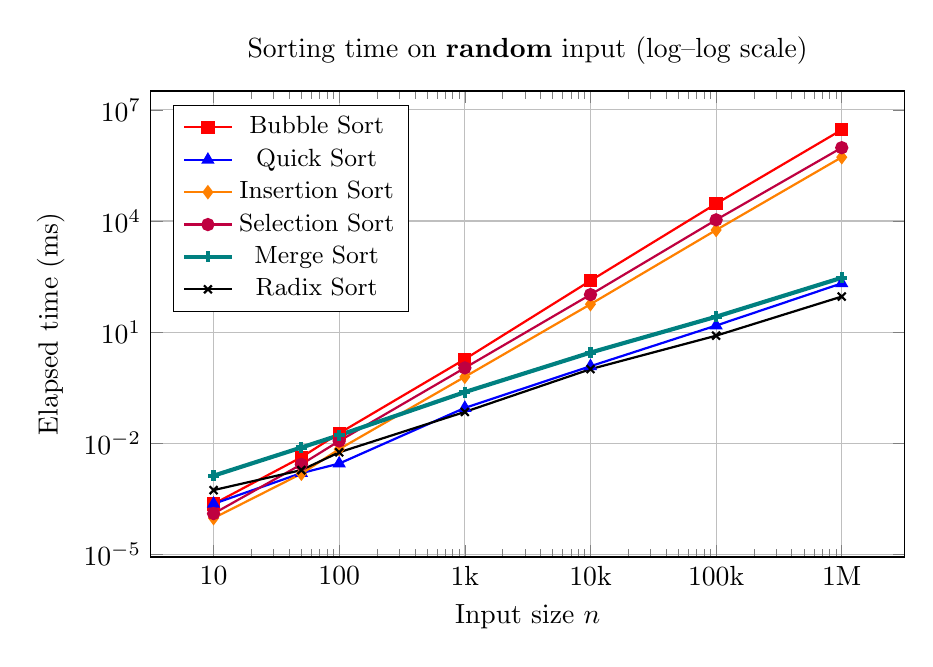
\begin{tikzpicture}
\begin{axis}[
  width=0.92\textwidth, height=7.5cm,
  xlabel={Input size $n$},
  ylabel={Elapsed time (ms)},
  xmode=log, ymode=log,
  xtick={10,100,1000,10000,100000,1000000},
  xticklabels={10, 100, 1k, 10k, 100k, 1M},
  legend pos=north west,
  legend style={font=\small},
  grid=major,
  title={Sorting time on \textbf{random} input (log--log scale)}
]
\addplot[color=red,   mark=square*,  thick] coordinates {
  (10,0.000229)(50,0.004181)(100,0.018632)(1000,1.860)(10000,244.2)(100000,29214)(1000000,2893099)
};
\addplot[color=blue,  mark=triangle*, thick] coordinates {
  (10,0.000231)(50,0.001562)(100,0.002826)(1000,0.090)(10000,1.2)(100000,15)(1000000,207)
};
\addplot[color=orange,mark=diamond*, thick] coordinates {
  (10,0.000095)(50,0.001501)(100,0.006928)(1000,0.620)(10000,56.6)(100000,5696)(1000000,526543)
};
\addplot[color=purple,mark=*,        thick] coordinates {
  (10,0.000126)(50,0.002686)(100,0.011483)(1000,1.080)(10000,102.7)(100000,10713)(1000000,950758)
};
\addplot[color=teal,  mark=+,        thick, line width=1.5pt] coordinates {
  (10,0.001329)(50,0.007665)(100,0.016482)(1000,0.240)(10000,2.8)(100000,26)(1000000,293)
};
\addplot[color=black, mark=x,        thick] coordinates {
  (10,0.000542)(50,0.001883)(100,0.005682)(1000,0.070)(10000,1.0)(100000,8)(1000000,91)
};
\legend{Bubble Sort, Quick Sort, Insertion Sort, Selection Sort, Merge Sort, Radix Sort}
\end{axis}
\end{tikzpicture}
\caption{Performance on random arrays across all sizes (log--log scale). Markers are used so the curves can be distinguished even without color.}
\label{fig:random}
\end{figure}

\begin{figure}[h!]
\centering
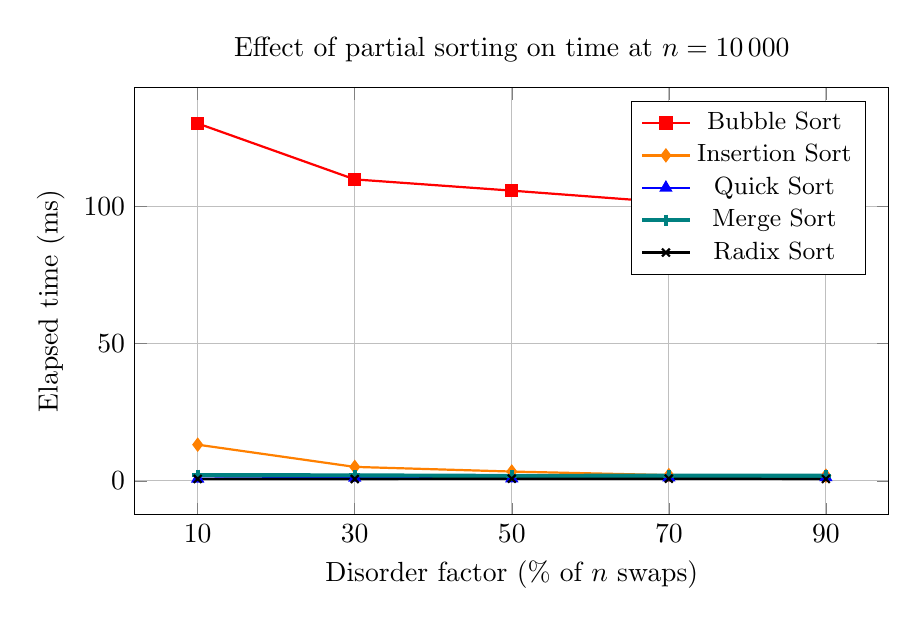
\begin{tikzpicture}
\begin{axis}[
  width=0.92\textwidth, height=7cm,
  xlabel={Disorder factor (\% of $n$ swaps)},
  ylabel={Elapsed time (ms)},
  xtick={10,30,50,70,90},
  legend pos=north east,
  legend style={font=\small},
  grid=major,
  title={Effect of partial sorting on time at $n=10\,000$}
]
\addplot[color=red,   mark=square*, thick] coordinates {
  (10,130.3)(30,109.9)(50,105.8)(70,101.5)(90,98.6)
};
\addplot[color=orange,mark=diamond*,thick] coordinates {
  (10,13.2)(30,5.1)(50,3.4)(70,2.1)(90,1.9)
};
\addplot[color=blue,  mark=triangle*,thick] coordinates {
  (10,0.8)(30,1.1)(50,0.9)(70,1.2)(90,1.3)
};
\addplot[color=teal,  mark=+, thick, line width=1.5pt] coordinates {
  (10,2.1)(30,2.0)(50,1.8)(70,1.9)(90,1.9)
};
\addplot[color=black, mark=x, thick] coordinates {
  (10,0.7)(30,0.7)(50,0.8)(70,0.8)(90,0.7)
};
\legend{Bubble Sort, Insertion Sort, Quick Sort, Merge Sort, Radix Sort}
\end{axis}
\end{tikzpicture}
\caption{Impact of disorder level on sorting time at $n=10\,000$. Marker shapes are used to distinguish algorithms without relying on color. Selection Sort omitted (flat at $\approx$100 ms).}
\label{fig:partial}
\end{figure}

\subsection{Key Observations}

\textbf{O1 -- Insertion Sort is very sensitive to input order}: On nearly-sorted data at $n=1\,000\,000$ (90\% factor), Insertion Sort takes 323 ms. This is close to Merge Sort (212 ms) and not far from Quick Sort (67 ms). On random data, the same algorithm takes 526\,543 ms. This difference of about 1600 times shows how much the input order can change the speed of an algorithm.

\textbf{O2 -- Radix Sort grows slowly with size}: When the input size increases 10 times (from $n=100\,000$ to $n=1\,000\,000$), Radix Sort on random data only increases about 11 times (from 8 ms to 91 ms). This matches its $O(dn)$ bound for a roughly constant number of digits $d$.

\textbf{O3 -- Quick Sort is reliable}: With median-of-three pivot selection, Quick Sort handles reversed arrays well (139 ms at $n=1\,000\,000$) and gives similar results across all input types. The slow $O(n^2)$ case is avoided.

\textbf{O4 -- Selection Sort always behaves the same}: No matter what the input looks like, Selection Sort always does $\binom{n}{2}$ comparisons. This means its time barely changes across input types. In systems where consistent timing is more important than speed, this can be useful.

\textbf{O5 -- Merge Sort is slow on small inputs}: At $n=10$, Merge Sort is the slowest algorithm (0.001329 ms/sort) even though it has good asymptotic complexity. The reason is that creating and freeing helper arrays for each merge adds a lot of overhead at small sizes. A good fix would be to switch to Insertion Sort below a certain threshold.

% ─── 5. Related Work ──────────────────────────────────────────────────────────
\section{Related Work}
\label{sec:related}

This section compares the present study with three relevant practical sources: McIlroy \cite{mcilroy1993}, Sedgewick and Wayne \cite{sedgewick2011}, and Bentley \cite{bentley1999}.

\paragraph{McIlroy's optimistic sorting perspective.}
McIlroy \cite{mcilroy1993} analyzes optimistic sorting techniques and how implementation choices such as pivot selection, partitioning strategy, and loop structure affect sort performance. His work is focused on practical, low-level tradeoffs in production-quality code.

The advantage of McIlroy over this paper is that he provides a deep engineering view of sorting implementations and explains how small changes can yield large real-world speedups.

The advantage of this paper over McIlroy is that it measures six different algorithms under a controlled partial-disorder model and reports timing results across seven input sizes up to $10^6$.

\paragraph{Sedgewick and Wayne's practical algorithm analysis.}
Sedgewick and Wayne \cite{sedgewick2011} offer a practical treatment of Quick Sort, Merge Sort, and Radix Sort, including empirical comparisons and guidance for implementation. Their text emphasizes how input characteristics and algorithm variants influence actual running time.

Their advantage is the broad survey of algorithmic variants and well-tested code patterns.

This paper's advantage is the narrower focus on partially sorted inputs with parameterized disorder and the inclusion of simpler algorithms such as Bubble Sort and Insertion Sort.

\paragraph{Bentley's nearly-sorted input work.}
Bentley \cite{bentley1999} discusses why adaptive methods like Insertion Sort and hybrid approaches such as Timsort perform well on nearly-sorted data. His work is a classic reference for choosing sorting strategies in systems that frequently see partially ordered inputs.

The advantage of Bentley over this paper is that he covers adaptive hybrid algorithms and production use cases.

The advantage of this paper is that it supplies direct timing data for a range of disorder levels, showing when simple algorithms remain competitive.

\paragraph{Theoretical foundation.}
Knuth \cite{knuth1998} and Cormen et al.\ \cite{cormen2022} provide the rigorous theoretical background for sorting complexity and lower bounds.

Their advantage is the depth of formal analysis, but they do not focus on the empirical effects of controlled partial disorder.

This paper therefore complements them by presenting experimental evidence on how input ordering affects modern sorting performance.

% ─── 6. Conclusions ───────────────────────────────────────────────────────────
\section{Conclusions and Future Work}
\label{sec:conclusions}

\subsection{Summary}

This paper compared six sorting algorithms --- Bubble Sort, Insertion Sort, Selection Sort, Quick Sort, Merge Sort, and Radix Sort --- using seven different input types and seven input sizes ranging over five orders of magnitude. The main findings are:

\begin{enumerate}[noitemsep]
  \item \textbf{For large general-purpose sorting}, Quick Sort and Radix Sort are the fastest. Radix Sort wins at $n=10^6$ on random data (91 ms vs.\ 207 ms for Quick Sort).
  \item \textbf{For nearly-sorted data}, Insertion Sort is as fast as $O(n \log n)$ algorithms and much faster at medium sizes.
  \item \textbf{Merge Sort} gives the most stable results across all input types, which makes it a good choice when you need consistent performance.
  \item \textbf{Selection Sort} is not affected by input order but is slow; it should not be used for $n \gtrsim 10^4$.
  \item \textbf{Bubble Sort} is only suitable for very small inputs or for teaching purposes.
\end{enumerate}

\subsection{Problems Encountered}

The main challenge was measuring time accurately for small array sizes. At $n=10$, a single sort takes just a few nanoseconds, which is below what \texttt{clock()} can measure. This was solved by running each test 1\,000\,000 times and averaging the result. At $n=10^6$, each test was only run once, so there is more variation in the results, but the times are large enough that this does not matter much.

\subsection{Future Work}

This study successfully built the benchmark and collected results across seven sizes and seven input variants. It did not yet test other data types or different computer systems, which are planned improvements.

\begin{itemize}[noitemsep]
  \item \textbf{Cache profiling}: Using tools like \texttt{perf} or \texttt{Valgrind/Cachegrind} to count cache misses, especially when comparing Merge Sort and Quick Sort.
  \item \textbf{Hybrid algorithms}: Testing Timsort and Introsort, which switch between algorithms depending on the input, and comparing them to the current results.
  \item \textbf{Parallel versions}: Running parallel Merge Sort and parallel Radix Sort on multi-core machines to see how CPU count affects speed.
  \item \textbf{Other data types}: Testing the algorithms on floating-point numbers, text strings, and other data types to see whether the same relative ordering holds.
  \item \textbf{Cross-machine comparison}: Running the benchmark on other computers with different CPUs and memory configurations to identify which hardware factors influence the results most.
\end{itemize}

% ─── 7. Bibliography ──────────────────────────────────────────────────────────
\label{sec:bibliography}

\bibliographystyle{plain}
\bibliography{references}

\appendix
\section{Pseudocode}
\label{app:pseudocode}

This appendix contains short, easy-to-understand pseudocode for the two main helper routines used in the benchmark.
\clearpage
\subsection{Partially sorted array generator}
\begin{lstlisting}[basicstyle=\ttfamily\small]
function generatePartiallySortedArray(n, factor):
    A = [0, 1, 2, ..., n-1]
    swaps = n / factor
    for i from 1 to swaps:
        a = random index in [0, n-1]
        b = random index in [0, n-1]
        swap(A[a], A[b])
    return A
\end{lstlisting}

\subsection{Median-of-three pivot selection}
\begin{lstlisting}[basicstyle=\ttfamily\small]
function choosePivot(A, low, high):
    mid = floor((low + high) / 2)
    sort the three values A[low], A[mid], A[high]
    return the median value
\end{lstlisting}

\end{document}

